\let\negmedspace\undefined
\let\negthickspace\undefined
\documentclass[journal]{IEEEtran}
\usepackage[a5paper, margin=10mm, onecolumn]{geometry}
%\usepackage{lmodern} % Ensure lmodern is loaded for pdflatex
\usepackage{tfrupee} % Include tfrupee package

\setlength{\headheight}{1cm} % Set the height of the header box
\setlength{\headsep}{0mm}     % Set the distance between the header box and the top of the text

\usepackage{gvv-book}
%\usepackage{gvv}
\usepackage{cite}
\usepackage{amsmath,amssymb,amsfonts,amsthm}
\usepackage{algorithmic}
\usepackage{graphicx}
\usepackage{textcomp}
\usepackage{xcolor}
\usepackage{txfonts}
\usepackage{listings}
\usepackage{enumitem}
\usepackage{mathtools}
\usepackage{gensymb}
\usepackage{comment}
\usepackage[breaklinks=true]{hyperref}
\usepackage{tkz-euclide} 
\usepackage{listings}
\usepackage{gvv}                                        
\def\inputGnumericTable{}                                 
\usepackage[latin1]{inputenc}                                
\usepackage{color}                                            
\usepackage{array}                                            
\usepackage{longtable}                                       
\usepackage{calc}                                             
\usepackage{multirow}                                         
\usepackage{hhline}                                           
\usepackage{ifthen}                                           
\usepackage{lscape}
\begin{document}

\bibliographystyle{IEEEtran}

\title{2.7.31}
\author{EE25BTECH11019 - Darji Vivek M.}
{\let\newpage\relax\maketitle}

\renewcommand{\thefigure}{\theenumi}
\renewcommand{\thetable}{\theenumi}
\setlength{\intextsep}{10pt}
\numberwithin{figure}{enumi}
\renewcommand{\thetable}{\theenumi}

\textbf{Question}:\\
Find the area of triangle $ABC$, whose vertices are $A(2,5)$, $B(4,7)$, and $C(6,2)$.
\hfill $\brak{12,2018}$

\solution \\[-2mm]

\begin{tabular}{|c|c|}
\hline
\textbf{Name} & \textbf{Value} \\ \hline
$\vec{A}$ & $\myvec{2 & 1 \\0 & 3}$ \\ \hline
\end{tabular}


\begin{align}
\vec{A} &= \myvec{2\\5}, \quad 
\vec{B} = \myvec{4\\7}, \quad 
\vec{C} = \myvec{6\\2}
\end{align}

\begin{align}
	\vec{A}-\vec{B}=\myvec{-2\\-2},\quad \vec{A}-\vec{C}=\myvec{-4\\3}
\end{align}
\begin{align}
	\brak{ABC}=\frac{1}{2}\norm{\brak{\vec{A}-\vec{B}}\times\brak{\vec{A}-\vec{C}}}=7
\end{align}

Hence, the area of $\triangle ABC$ is $\textbf{7}$.

\begin{figure}[H]
\centering
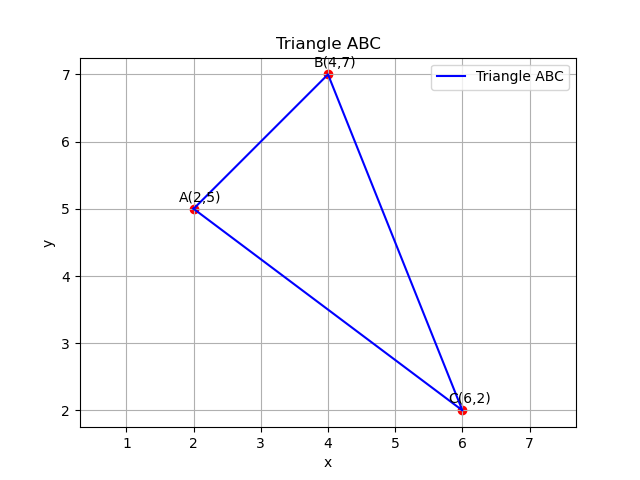
\includegraphics[width=0.75\columnwidth]{figs/triangle.png}
\caption{Triangle $ABC$ with vertices A(2,5), B(4,7), C(6,2)}
\label{fig:2.7.31}
\end{figure}

\end{document}